\frame[plain]{\titlepage}
\frame{\frametitle{Outline}\tableofcontents}

\section{Introduction}

\begin{frame}
    \frametitle{Latex and Beamer}
    
    LaTeX is a high-quality typesetting system; 
    it includes features designed for the production of 
    technical and scientific documentation.

    \vspace{0.4cm}

    \pause

    Beamer is a LaTeX class to create powerful, 
    flexible and nice-looking presentations and slides. 
    
    The beamer class is focussed on producing (on-screen) presentations, 
    along with support material such as handouts and speaker notes.
    
\end{frame}

\section{Beamer Basic}
\subsection{Hightlight}

\begin{frame}
    \frametitle{Block and Alert}

    \begin{block}{Pythagorean theorem}
        \vspace*{-\baselineskip}\setlength\belowdisplayshortskip{0.6pt}
        $$a^2 + b^2 = c^2$$
        % \vspace*{-\baselineskip}\setlength\belowdisplayshortskip{0.1pt}
        where c represents the length of the hypotenuse and 
        a and b the lengths of the triangle's other two sides.
    \end{block}
    
    \begin{alertblock}{Remark}
        \begin{itemize}
            \item the environment above is \alert{block}
            \item the environment here is \alert{alertblock}
        \end{itemize}
    \end{alertblock}

\end{frame}

\begin{frame}
    \frametitle{Proof}

    \begin{block}{Pythagorean theorem}
        \vspace*{-\baselineskip}\setlength\belowdisplayshortskip{0.1pt}
        $$a^2 + b^2 = c^2$$
        % \vspace*{-\baselineskip}\setlength\belowdisplayshortskip{0.2pt}
    \end{block}
    
    \vspace{0.4cm}

    \begin{proof}
        \vspace*{-\baselineskip}\setlength\belowdisplayshortskip{0pt}
        \begin{align*}
            &3^2 + 4^2 = 5^2\\
            &5^2 + 12^2 = 13^2
        \end{align*}
        % \vspace*{-\baselineskip}\setlength\belowdisplayshortskip{0pt}
    \end{proof}
    
\end{frame}

\subsection{Other Environments}

\begin{frame}{Algorithm}
    
    \begin{algorithm}[H]
        \KwData{this text}
        \KwResult{how to write algorithm with \LaTeX2e }
        initialization\;
        \While{not at end of this document}{
            read current\;
            \eIf{understand}{
            go to next section\;
            current section becomes this one\;
            }{
            go back to the beginning of current section\;
            }
        }
        \caption{How to write algorithms
        (copied from \href{https://en.wikibooks.org/wiki/LaTeX/Algorithms}{here})}
        \end{algorithm}
\end{frame}

\begin{frame}{More}

    More environments such as

    \begin{itemize}
        \item Definition
        \item lemma
        \item corollary
        \item example
    \end{itemize}
    
\end{frame}

\section{Beamer More}

\subsection{Split Screen}

\begin{frame}{Minipage}
    \begin{minipage}{0.5\linewidth}
        \begin{figure}[h]
            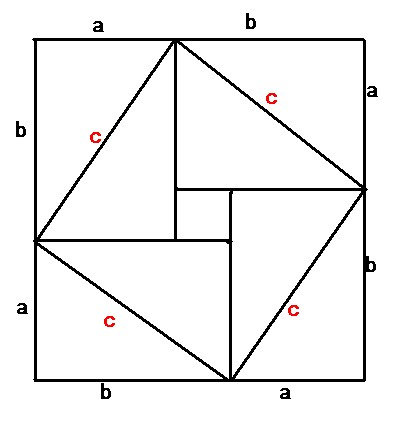
\includegraphics[width=\textwidth]{imgs/pythagorean.jpg}
        \end{figure}
    \end{minipage}%
    \hfill
    \begin{minipage}{0.4\linewidth}
        \begin{enumerate}
            \item item
            \item another
            \item more
            \begin{itemize}
                \item first
                \item second
                \item third
            \end{itemize}
        \end{enumerate}
    \end{minipage}
    
\end{frame}

\begin{frame}{Columns}
    \begin{columns}
        \column{0.5\textwidth}
        This is a text in first column.
        $$E=mc^2$$
        \begin{itemize}
        \item First item
        \item Second item
        \end{itemize}
        
        \column{0.5\textwidth}
        \begin{block}{first block}
            columns achieves splitting the screen
        \end{block}
        \begin{block}{second block}
            stack block in columns
        \end{block}
        
    \end{columns}
\end{frame}

\subsection{Table}


\begin{frame}{Create Tables}
    \begin{center}
        \begin{table}[!t]  
            % \caption{Three line}
            % \label{table_time}
            \begin{tabular}{ccc}  
                \toprule   
                first&second&third\\ 
                \midrule       
                1 & 2 & 3 \\ 
                4 & 5 & 6 \\ 
                7 & 8 & 9 \\
                \bottomrule  
            \end{tabular}
        \end{table}
    \end{center}
\end{frame}



\section{Conclusion}

\begin{frame}{End}
    The last page.
\end{frame}